\normalfont\documentclass[letterpaper,11pt]{article}
\usepackage{amsmath, amsfonts,amssymb,latexsym}
\usepackage{fullpage}
\usepackage{parskip}
\usepackage{flexisym}
\usepackage{indentfirst}
\usepackage{algorithm}
\usepackage{algorithmicx}
\usepackage{hyperref}
\usepackage{algpseudocode}
\usepackage{graphicx}
\begin{document}
\setlength{\parindent}{2ex}
\newcommand{\header}{
	\noindent \fbox{
	\begin{minipage}{6.4in}
	\medskip
	\textbf{CS 260 Fundamentals of the Design and Analysis of Algorithms} \hfill \textbf{Fall 2016} \\[1mm]
	\begin{center}
		{\Large HomeWork 6} \\[3mm]
	\end{center}
	  Name: \itshape{Liangjian Chen} \\
	  \textnormal{ID}: \itshape{\#52006933} \hfill \today
	\medskip
	\end{minipage}}
}
\bigskip
\header
In this homework, $build(x,y,c)$ means build a edge from $x$ to $y$ which capacity $c$.
$s$ is the source, $t$ is the sink.
\begin{enumerate}
\item [Problem 6]\textbf{Solution:}\par
	Consider a bipartite graph, left part is fixture, right part is switch. For every pair of fixture and switch, draw a line segment between these two point, and test whether it intersects with any boundary segment. If it does not intersect with any boundary then we draw an edge between these two points.\par
	Next, run the bipartite graph matching algorithm. If the result is $n$ then it is possible to make such an arrangement. Otherwise it does not.
\item [Problem 7]\textbf{Solution:}\par
	for every client $c_i$, $build(s,c_i,1)$. for every base station$b_i$ $build(b_i,t,L)$. for every pair of client$c_i$ and base station $b_j$. If $c_i$ can connect to $b_j$ then $build(c_i,b_j,1)$. Then run the maximum flow algorithm. If the result is same as the number of clients, then all clients can be assigned to a base station.
\item [Problem 8]\textbf{Solution:}\par
	\begin{enumerate}
	\item
	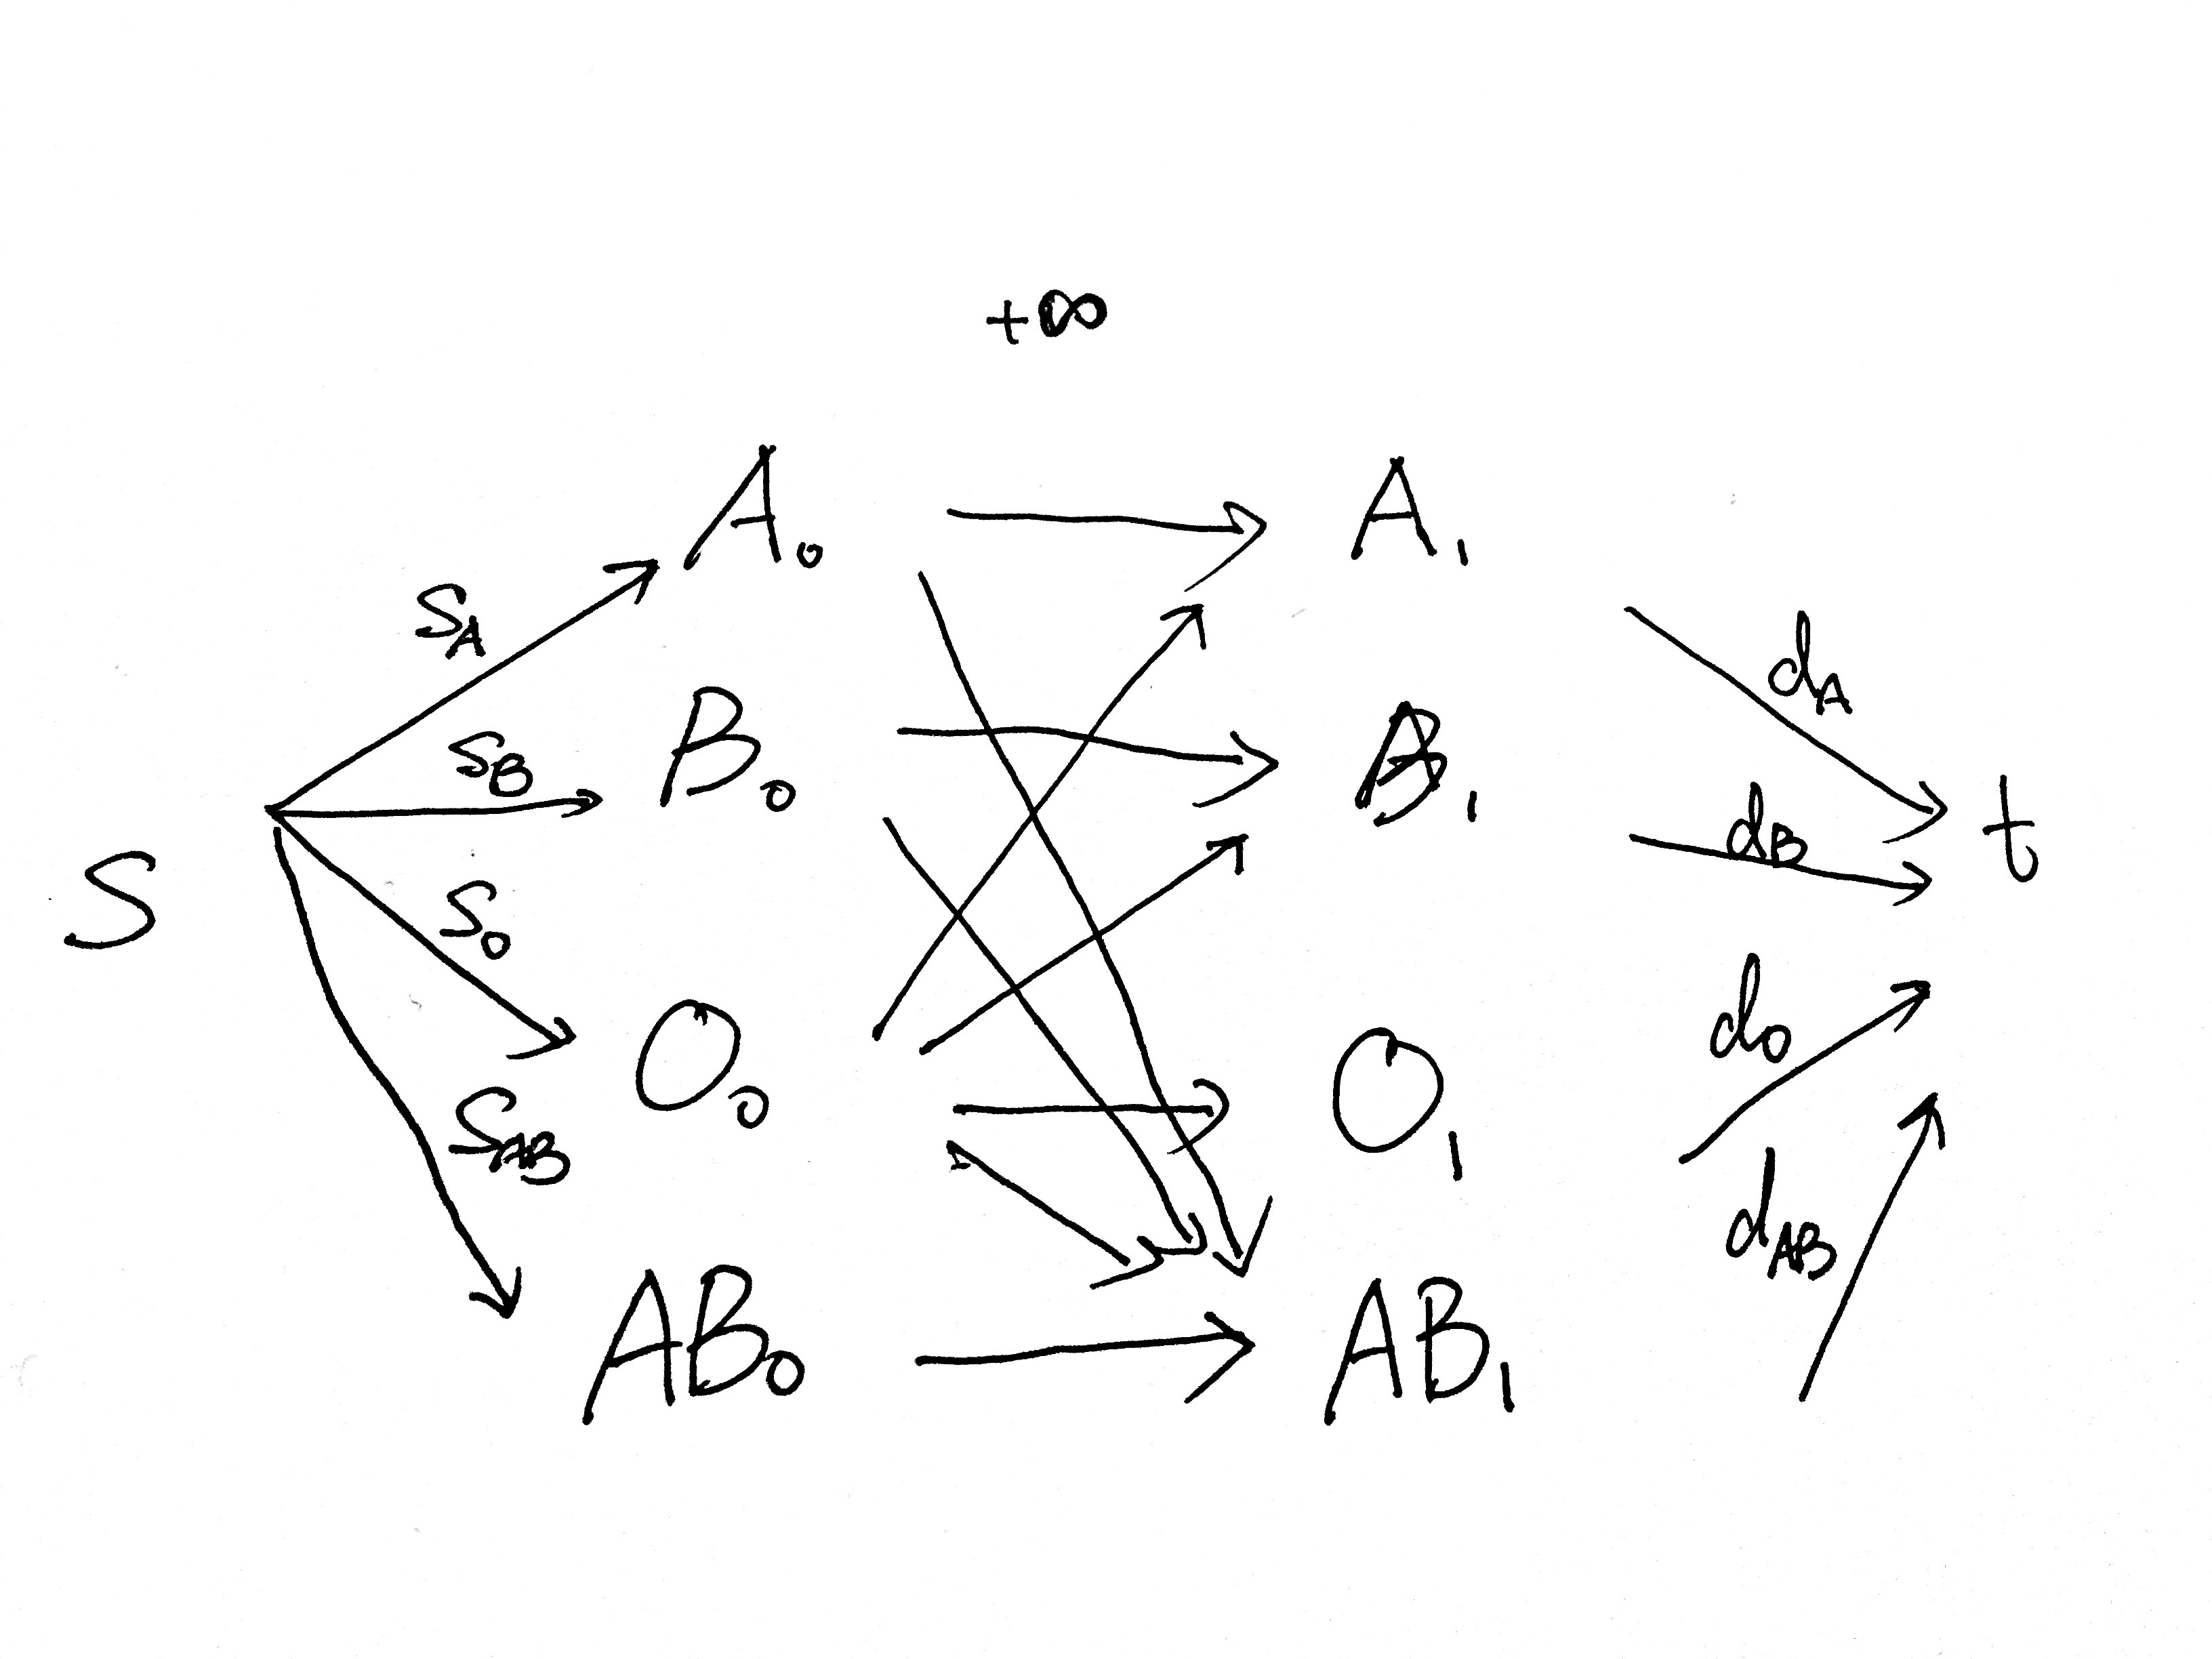
\includegraphics[width = 4in]{1.JPG}\par
	Run maximum flow algorithm on above graph. If $d_A+d_B+d_O+d_{AB}$ = Maximum flow then it is sufficient.
	\item
		Maximum is 99. All B,AB patient will be served and one of A patient or one of O patient could not get the blood.\par
		Explain:
		the supply of A and O is 86, but the demand of A and O is 87. So at least a patient of type A or O can not be served.
	\end{enumerate}
\item [Problem 9]\textbf{Solution:}\par
	for every injured people$p_i$, $build(s,p_i,1)$, for every hospital $h_i$, $build(h_i,t,\lceil \frac{n}{k}\rceil)$. Then for every pair of people$p_i$ and hospital$h_j$, $build(p_i,h_j,1)$.
	If the result is $n$, then it is possible.
\item [Problem 10]\textbf{Solution:}\par
	Assume that $e^*$ connects $u$ and $v$. 
	If $e^*$ is not in the cut, then the maximum flow does not change.\par
	Otherwise, in the residual network. Think about now we set $t$ as a new source and $s$ as a new sink. Then finding a path from $t$ to $v$, and a path $u$ to $s$. and reduce all the flow in this path by one.
\item [Problem 11]\textbf{Solution:}\par
	No, it is not.For any positive integer number $n$, construct the follow network(all edges' capacity is $1$).\par
	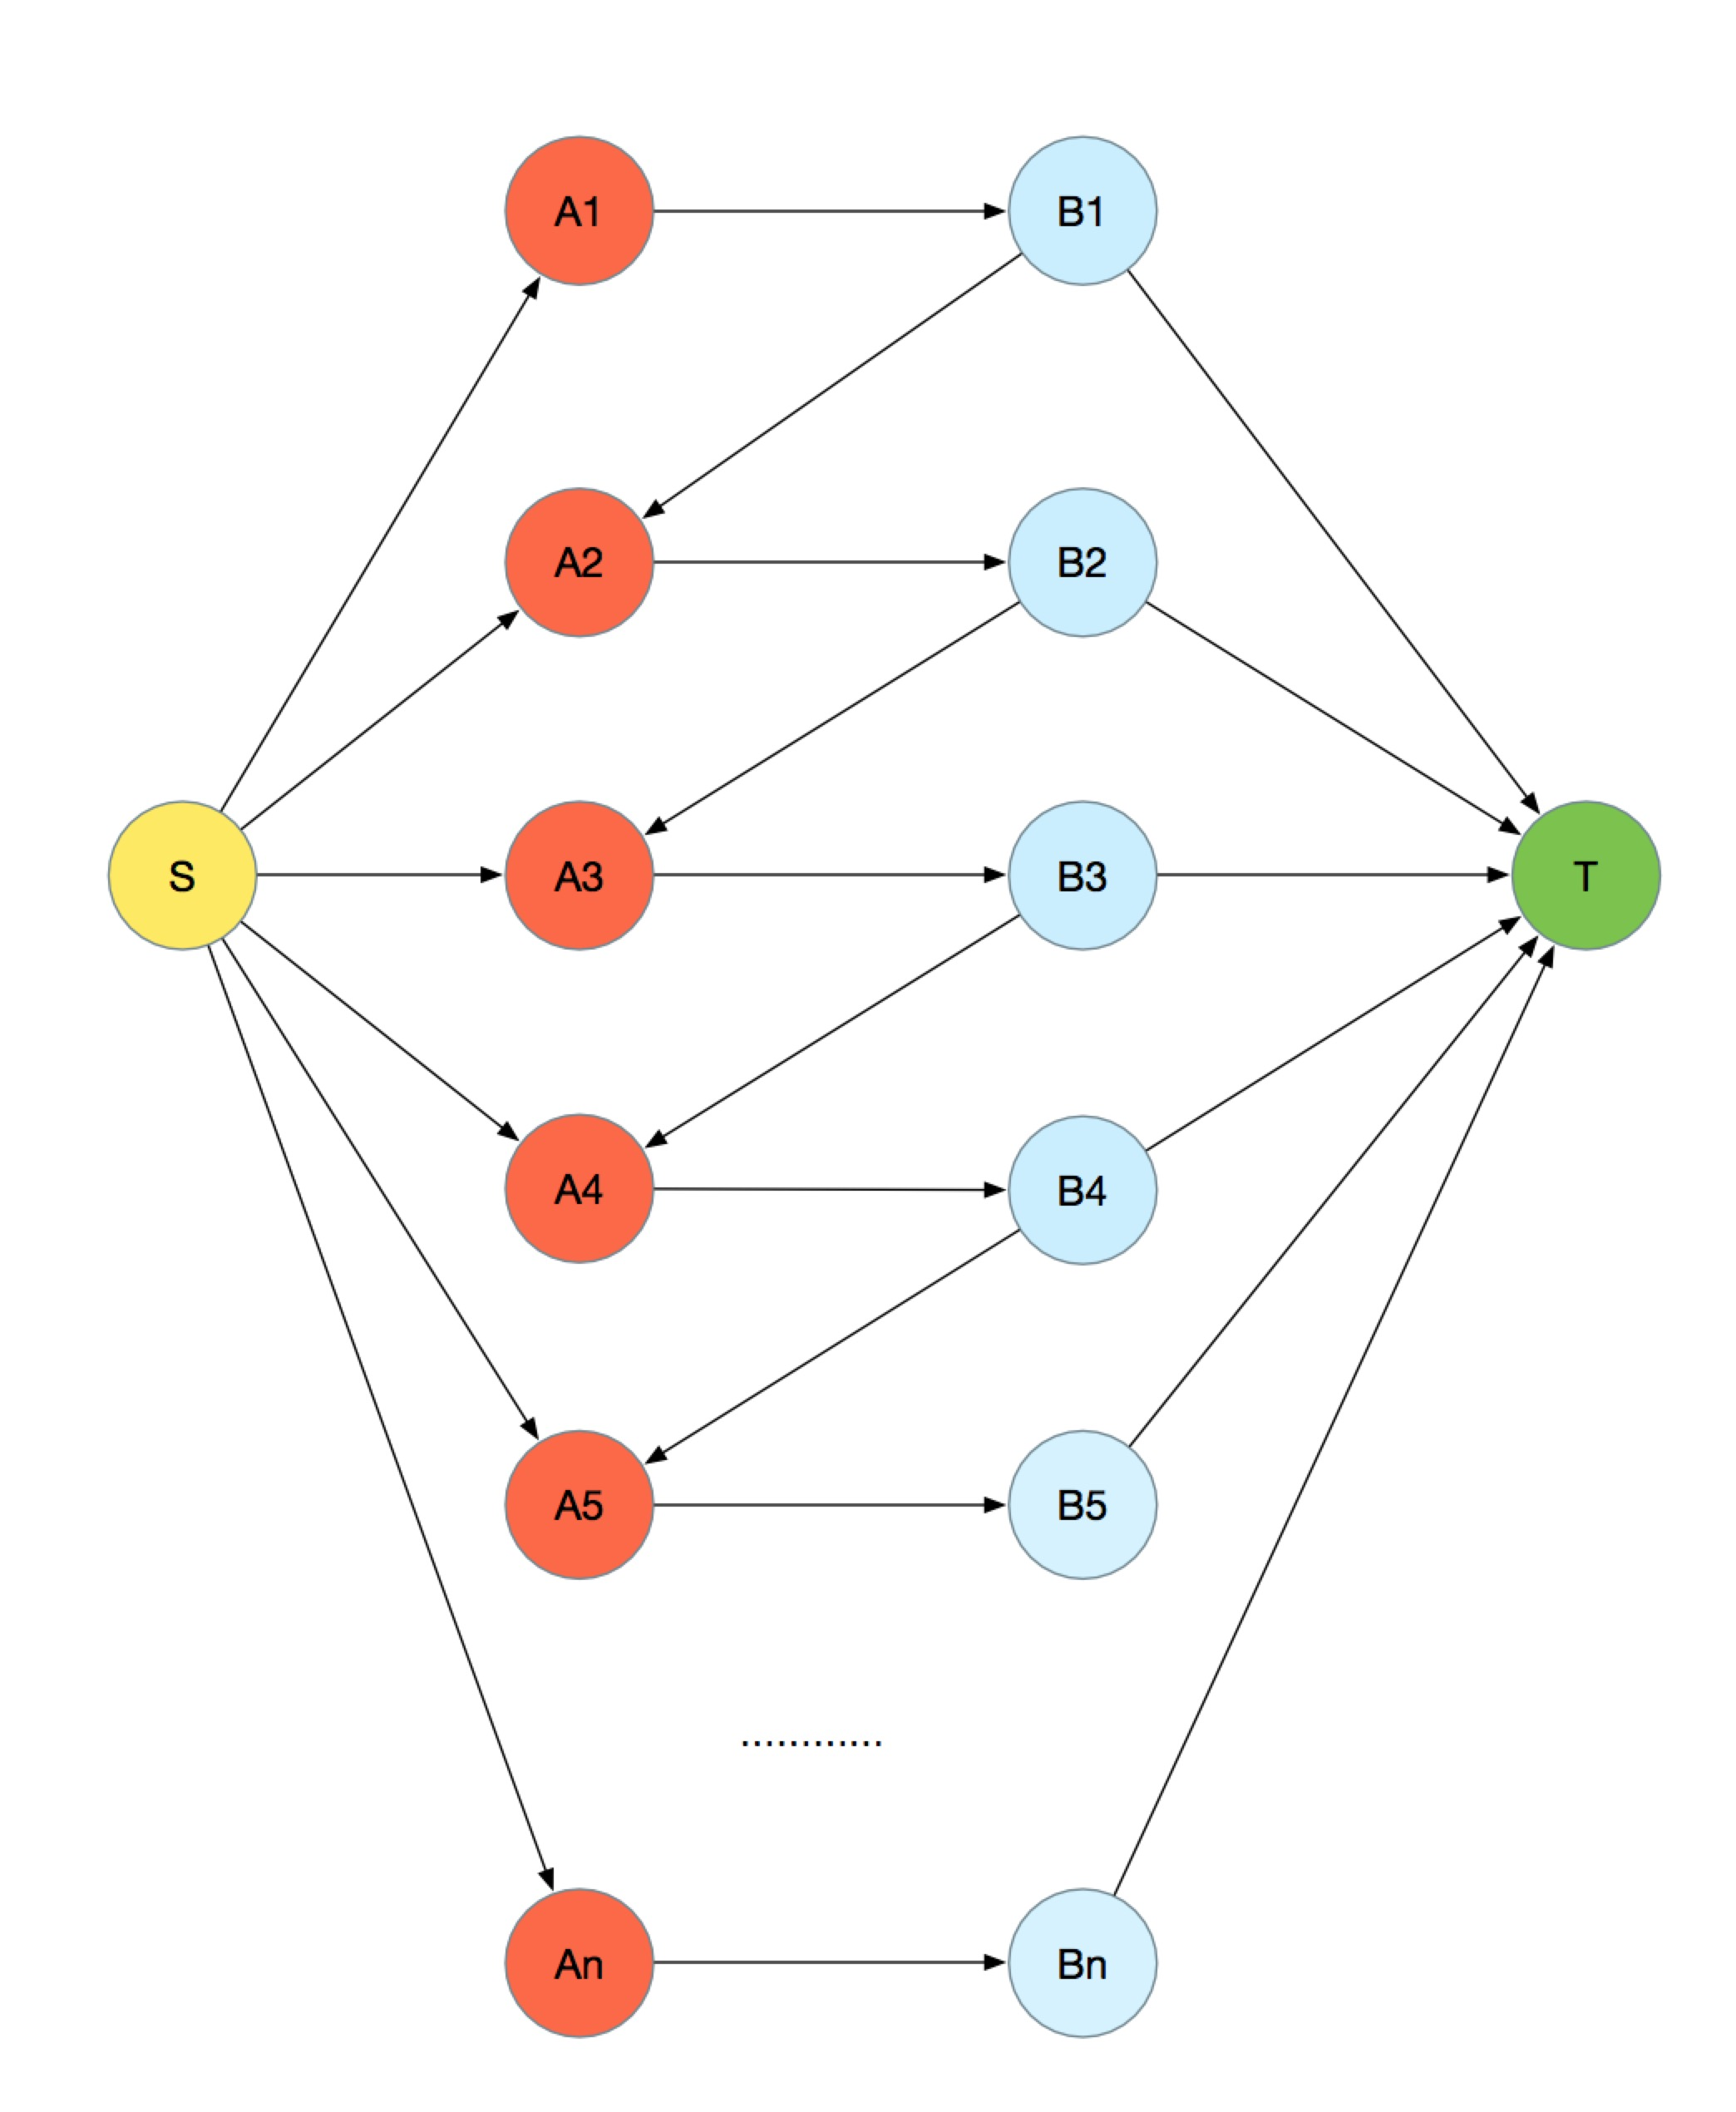
\includegraphics[width = 4in]{2.jpeg}\par
	In this network, apparently the maximum flow is $n$. But if we find the augment path $s\to A_1 \to B_1 \to A_2 \to B_2 \to ... \to A_n \to B_n \to t$ first. Then we can not find any other augment path if we use the algorithm mentioned in the question. Thus the ratio is $\frac{1}{n}$. Because $n$ could be any larger positive number, so there is no such $b$.
\item [Problem 24]\textbf{Solution:}\par
	Run the maximum flow algorithm in the original network. Then in the residual network, if one edge is not full, called it valid. Starting from the $s$, find the node set that can be reached from $s$ through valid edge and call it set $\mathcal{S}$. From $t$ find the node set that can be reached to the $t$ through valid edge call it $\mathcal{T}$. If $|\mathcal{S}| + |\mathcal{T}| = n$ then, it is a unique cut. Otherwise it is not.
\end{enumerate}
\end{document}
